\section{Probability}

Probability is used to model real-life events and their likelihoods with mathematical tools.

When dealing with probabilities, we want to consider a random process and its possible outcomes. For instance, rolling a dice is a random process that produces six outcomes.

\begin{figure}[H]
    \centering

    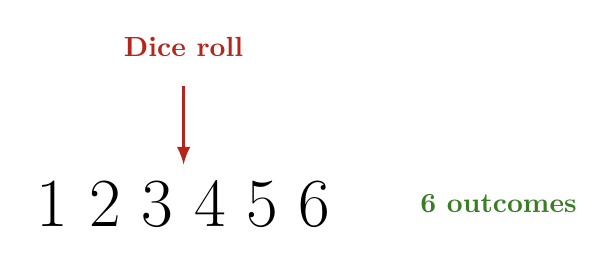
\begin{tikzpicture}
        \node[BrickRed] at (0, 2) {
            \textbf{Dice roll}
        };

        \draw[-latex, very thick, BrickRed] (0, 1.5) -- (0, 0.5);

        \node at (0, 0) {
            \Huge
            \dice{1}
            \dice{2}
            \dice{3}
            \dice{4}
            \dice{5}
            \dice{6}
        };

        \node[OliveGreen] at (4, 0) {
            \textbf{6 outcomes}
        };
    \end{tikzpicture}
    
    \caption{Rolling a dice is a random process that generates six possible outcomes.}
    \label{fig:Ch09-rolling-dice}
\end{figure}

The set of all possible outcomes is called the \textit{sample space} or \textit{universe}, which we denote by \(\Omega\).
%
\[\Omega = \{
    \text{rolling } 1,\;
    \text{rolling } 2,\;
    \text{rolling } 3,\;
    \text{rolling } 4,\;
    \text{rolling } 5,\;
    \text{rolling } 6
\}\]
%
Any subset of \(\Omega\) is called an event. For example, events associated with rolling a dice include the following.
%
\begin{align*}
    A &= \{2, 4, 6\} \tag{rolling an even number}\\
    B &= \{1, 3, 5\} \tag{rolling an odd number}\\
    C &= \{5, 6\} \tag{rolling a number greater than 4}
\end{align*}
%
This allows us to treat events as sets:
%
\begin{align*}
    \text{``Rolling an even number greater than 4''} &= A \cap C \tag{intersection}\\
    \text{``Rolling a number that is odd or greater than 4''} &= B \cup C \tag{union}\\
    \text{``Rolling a number not greater than 4''} &= \overline{C} \tag{complement}\\
    \text{``Rolling an odd number not greater than 4''} &= B \setminus C \tag{minus}
\end{align*}
%
(The complement of a set \(S\) is also sometimes denoted as \(A^c\), but here we will stick to the notation \(\overline{S}\).)

We say that two events \(A\) and \(B\) are \textit{disjoint} if and only if their intersection is the empty set.
%
\[A \cap B = \emptyset\]


\subsection{Probability laws}

We represent the likelihood of an event \(E\) using its probability \(P(E)\). We have the following laws.
%
\begin{align*}
    P(A) &\geq 0 \tag{probabilities are non-negative}\\
    P(\Omega) &= 1 \tag{whole sample space has probability 1}\\
    P(A \cup B) &= P(A) + P(B) \text{\hspace{1em} if \(A, B\) disjoint} \tag{additivity}
\end{align*}
%
This has several consequences, which we will prove below. (Drawing set diagrams are really useful in constructing these proofs.)

\vspace{15pt}
\begin{mdframed}[linewidth=1pt]
\noindent \textbf{Theorem.} If \(A \subseteq B\), then \(P(A) \leq P(B)\).

\textbf{Intuition.} Event \(B\) ``includes'' event \(A\).

\textbf{Proof.} Assume \(A \subseteq B\). Let \(C = B \setminus A\). Since \(A\) and \(C\) are disjoint, we have
%
\begin{align*}
    P(B) &= P(A \cup C) \tag{by definition}\\
    &= P(A) + P(C) \tag{by additivity}\\
    &\geq P(A)\text{.} \tag{\(P(C)\) must be non-negative}
\end{align*}
%
Hence proved.
\end{mdframed}
\vspace{15pt}


\vspace{15pt}
\begin{mdframed}[linewidth=1pt]
\noindent \textbf{Theorem.} \(P(A \cup B) = P(A) + P(B) - P(A \cap B)\).

\textbf{Proof.} Let \(A' = A \setminus B\) and \(B' = B \setminus A\). It follows that
%
\begin{align*}
    \text{RHS} &= P(A) + P(B) - P(A \cap B)\\
    &= P(A) + P(B' \cup (A \cap B)) - P(A \cap B)\\
    &= P(A) + P(B') + P(A \cap B) - P(A \cap B) \tag{\(B'\) and \(A \cap B\) are disjoint}\\
    &= P(A) + P(B')\\
    &= P(A \cup B') \tag{\(A\) and \(B'\) are disjoint}\\
    &= P(A \cup B)\\
    &= \text{LHS}
\end{align*}
%
Hence proved.
\end{mdframed}
\vspace{15pt}



\vspace{15pt}
\begin{mdframed}[linewidth=1pt]
\noindent \textbf{Theorem.} \(P(\overline{A}) = 1 - P(A)\).

\textbf{Proof.} Since \(A\) and \(\overline{A}\) are disjoint, we have
%
\begin{align*}
    P(A \cup \overline{A}) &= P(A) + P(\overline{A})\\
    P(\Omega) &= P(A) + P(\overline{A})\\
    1 &= P(A) + P(\overline{A})\\
    P(\overline{A}) &= 1 - P(A)
\end{align*}
%
Hence proved.
\end{mdframed}
\vspace{15pt}



\subsection{Discrete probabilities}

A set is said to be \textit{countable} if it is finite or in bijection with \(\mathbb{N}\).

If the sample space of a random process is countable, then we can measure probabilities in that space as a sum.
%
\[P(A) = \sum_{a \in A}\; P(\{a\})\]
%
This is a direct consequence of the law of additivity for disjoint events.


\subsubsection{Example: Finite sample spaces}

For example, for our example of dice rolling, let \(C\) be the event of rolling a number greater than \(4\). This event consists of two possible outcomes: rolling a \(5\) and rolling a \(6\). Therefore,
%
\begin{align*}
    P(C) &= P(\{
        \text{rolling } 5,\;
        \text{rolling } 6
    \})\\
    &= P(\{\text{rolling } 5\})
    + P(\{\text{rolling } 6\})\\
    &= \frac{1}{6} + \frac{1}{6}\\
    &= \frac{1}{3}
\end{align*}

Furthermore, in the case where \(\Omega\) has a finite size \(n\) with every outcome equally likely (e.g. dice rolling), we can express the probability of any event \(A\) as
%
\[P(A) = \frac{\abs{A}}{n}\text{.}\]
%
This streamlines the calculation of \(P(C)\) above as follows.
%
\[
    P(C) = P(\{
        \text{rolling } 5,\;
        \text{rolling } 6
    \})
    = \frac{2}{6} = \frac{1}{3}
\]


\subsubsection{Countably infinite sample spaces}

Now consider a different scenario with an infinite, but nevertheless countable sample space.

\begin{quote}
    A fair coin is tossed repetitively until heads is observed. The number of coin tosses is recorded as the outcome of this experiment. The sample space \(\Omega\) of this process is thus \(\mathbb{N}\), which is countably infinite.
    
    Verify that \(P(\Omega) = 1\).
\end{quote}

Since the sample space is countably infinite, we can express \(P(\Omega)\) as an infinite sum.
%
\begin{align*}
    P(\Omega) &= \Sigma_{a \in \Omega}\; P(\{a\})\\
    &= P(\{1\}) + P(\{2\}) + P(\{3\}) + \cdots\\
    &= P(\text{First head on toss \#1}) + P(\text{First head on toss \#2}) + P(\text{First head on toss \#3}) + \cdots\\
    &= \frac{1}{2} + \frac{1}{2} \times \frac{1}{2} + \frac{1}{2} \times \frac{1}{2} \times \frac{1}{2} + \cdots\\
    &= \sum_{k\geq 1} \frac{1}{2^k}\\
    &= 1 \tag{geometric series}
\end{align*}



\subsection{Continuous probabilities}

If the sample space is instead \textit{uncountable} (e.g. intervals of \(\mathbb{R}\)), then we can only measure probabilities as a continuous sum, i.e. an integral.

For example, consider a random number \(x\) in the interval \([0, 1]\). The probabiliy that \(x\) is strictly higher than \(0.7\) is given by
%
\[P(x > 0.7) = \int_{0.7}^{1} dx = 0.3\text{.}\]


\subsection{Conditional probabilities}

